%%%%%%%%%%%%%%%%%%%%%%%%%%%%%%%
\tikzset{global scale/.style={
    scale=#1,
    every node/.append style={scale=#1}
  }
}

\pgfplotsset{
   width=0.4\textwidth,
   height=0.25\textheight,
   grid=major,
   % grid style=dashed,
   major grid style={dotted},
   symbolic x coords={0,0.1,0.2,0.3,0.4,0.5,0.6,0.7,0.8,0.9,1.0},
   enlarge y limits={upper,value=0.05},
   legend style={
      fill,
      at={(0.50,16.5em)},
      legend columns=3,
      legend cell align=left,
      anchor=south
      },
   }
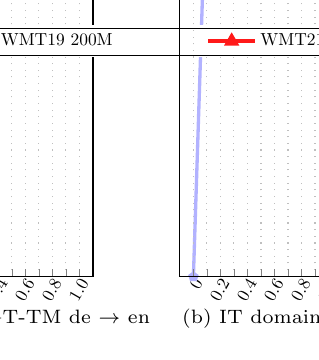
\begin{tikzpicture}
%%%%%%%%%%%%%%%%%%%%%%%%%%%%%%%%%%%%%%%%%%  
\useasboundingbox (13em,-1em) rectangle (3.5em,10em);
%%%%%%%%%%%%%%%%%%%%%%%%%%%%%%%%%%%%%%%%%%%%%%
\begin{axis}[
global scale = 0.63,
   at={(0,1em)},
   xtick pos=left,
   axis y line*=right,
   % ybar,
   % ymajorgrids,
   bar width=0.2cm,
   ymin=0, ymax=1.000,
   ytick={0,0.25,0.50,0.75,1.00},
   xtick={0,0.1,0.2,0.3,0.4,0.5,0.6,0.7,0.8,0.9,1.0},
   xticklabels={0,,0.2,,0.4,,0.6,,0.8,,1.0},
   yticklabels={,,,,},
   % xlabel={(a)DGT de$\rightarrow$en},
   ylabel style={align=center},
   % ylabel={TM FMS ratio},
   % ylabel style={rotate=180},
   xtick=data,
   xticklabel style={
      inner sep=0pt,
      anchor=north east,
      rotate=60
      },
    yticklabel style={/pgf/number format/fixed,/pgf/number format/fixed zerofill,/pgf/number format/precision=2,rotate=-90}
   ]              
       % 相似度
   \addplot[very thick,draw=blue!90,mark=pentagon*,mark color=blue!30,color=blue!30] plot coordinates {
      (0,0) (0.1,0.0027) (0.2,0.0357)
      (0.3,0.1747) (0.4,0.299) (0.5,0.3747)
      (0.6,0.466) (0.7,0.5556) (0.8,0.6382)
      (0.9,0.7592) (1.0,1)
      };\label{B1}                 
\end{axis}
\begin{axis}[
global scale = 0.63,
   at={(0,1em)},
    legend entries={WMT19 200M},
    ymajorgrids=true,
    xmajorgrids=true,
    legend style={draw=none,
    line width=1pt,
    at={(5em,12.5em)},
    anchor=south},
   axis y line*=left,
   xticklabels={},
   ymin=20.00, ymax=70.00,
   ytick={20.00,32.50,45.00,57.5,70},
   % ylabel={BLEU},
   yticklabel style={/pgf/number format/fixed,/pgf/number format/fixed zerofill,/pgf/number format/precision=2,rotate=90}
   ]
   % \addlegendimage{/pgfplots/refstyle=A}
   % \addlegendentry{Nombre de données (Golden)}
   % \addlegendimage{draw=blue!60,/pgfplots/refstyle=B}
   % \addlegendentry{DGT-de$\rightarrow$en}
   % DGT WMT19
   \addplot[very thick,draw=red!20,mark=square*,mark color=red!20,color=red!20] plot coordinates{
      (0,66.90)(0.1,66.90) (0.2,66.88)
      (0.3,66.34) (0.4,65.63) (0.5,64.30)
      (0.6,62.70) (0.7,61.04) (0.8,58.45)
      (0.9,54.15) (1.0,44.21)
      };
   % \addlegendentry{WMT19}
   % DGT WMT21
   \addplot[very thick,draw=red!90,mark=triangle*,mark color=red!90,color=red!90] plot coordinates {
      (0,66.90) (0.1,66.90) (0.2,67.06)
      (0.3,67.02) (0.4,66.74) (0.5,65.84)
      (0.6,64.58) (0.7,63.08) (0.8,60.59)
      (0.9,57.33) (1.0,49.21)
      };
   % \addlegendentry{WMT21}
   \end{axis}
\node at (4em,-0.5em){\scriptsize (a) DGT-TM de $\rightarrow$ en};
\node at (13.2em,-0.5em){\scriptsize (b) IT domain de $\rightarrow$ en};
%%%%%%%%%%第二个图%%%%%%%%%%%%%%%%%%%%5
\begin{axis}[
global scale = 0.63,
   at={(9em,1em)},
   xtick pos=left,
   axis y line*=right,
   % ybar,
   % ymajorgrids,
   bar width=0.2cm,
   ymin=0, ymax=1.000,
   xticklabels={0,,0.2,,0.4,,0.6,,0.8,,1.0},
   ytick={0,0.250,0.5,0.750,1.000},
   yticklabels={0,0.25,0.50,0.75,1.00},
   % xlabel={(b)IT de$\rightarrow$en},
   ylabel style={align=center},
   % ylabel={proportion},
   ylabel style={rotate=180},
   xtick=data,
   xticklabel style={
      inner sep=0pt,
      anchor=north east,
      rotate=60
      },
    yticklabel style={/pgf/number format/fixed,/pgf/number format/fixed zerofill,/pgf/number format/precision=3,rotate=-90}
   ]   
   %%%%%相似度%%%%%%%
   \addplot[very thick,draw=blue!90,mark=pentagon*,mark color=blue!30,color=blue!30] plot coordinates {
      (0,0) (0.1,0.062) (0.2,0.134)
      (0.3,0.2115) (0.4,0.314) (0.5,0.387)
      (0.6,0.598) (0.7,0.76) (0.8,0.8565)
      (0.9,0.9425) (1.0,1)
      };\label{B2}                
\end{axis}
\begin{axis}[
global scale = 0.63,
    at={(9em,1em)},
    % legend entries={WMT19,WMT21},
       legend entries={,WMT21 4B},
    ymajorgrids=true,
    xmajorgrids=true,
    legend style={draw=none,
    line width=1pt,
    at={(5em,12.5em)},
    anchor=south},
   axis y line*=left,
   xticklabels={},
   ymin=20.00, ymax=70.00,
   ytick={20.00,32.50,45.00,57.5,70},
   yticklabels={,,,,},
   % ylabel={BLEU},
   yticklabel style={/pgf/number format/fixed,/pgf/number format/fixed zerofill,/pgf/number format/precision=2,rotate=90}
   ]
   % \addlegendimage{/pgfplots/refstyle=A}
   % \addlegendentry{Nombre de données (Golden)}
   % \addlegendimage{draw=blue!60,/pgfplots/refstyle=B}
   % \addlegendentry{DGT-de$\rightarrow$en}
   % IT WMT19
   \addplot[very thick,draw=red!20,mark=square*,mark color=red!20,color=red!20] plot coordinates{
      (0,47.46)(0.1,44.48) (0.2,43.85)
      (0.3,43.30) (0.4,40.78) (0.5,36.92)
      (0.6,35.78) (0.7,32.55) (0.8,29.27)
      (0.9,28.17) (1.0,26.25)
      };
   % \addlegendentry{WMT19}
   % IT WMT21
   \addplot[very thick,draw=red!90,mark=triangle*,mark color=red!90,color=red!90] plot coordinates {
      (0,47.46) (0.1,44.01) (0.2,43.19)
      (0.3,42.31) (0.4,37.53) (0.5,34.35)
      (0.6,33.31) (0.7,30.17) (0.8,27.23)
      (0.9,26.25) (1.0,24.90)
      };
   % \addlegendentry{WMT21}
   \end{axis}
   \node [rectangle,draw=black,inner sep=2pt,minimum height=1em,minimum width=16.87em,font=\small,anchor=north,align=center] (final) at (8.4em,10.0em){};
   \node  [rotate=90] at(-1.3em,5em){\scriptsize BLEU};
   \node  [rotate=270] at(18.2em,5em){\scriptsize proportion};
\end{tikzpicture}